\documentclass[conference]{IEEEtran}
\IEEEoverridecommandlockouts
% The preceding line is only needed to identify funding in the first footnote. If that is unneeded, please comment it out.
\usepackage{cite}
\usepackage{amsmath,amssymb,amsfonts}
\usepackage{algorithmic}
\usepackage{graphicx}
\usepackage{textcomp}
\usepackage{xcolor}
\usepackage{multirow}
\usepackage{float}
\usepackage{caption}
\usepackage{tikz}
\captionsetup[table]{skip=10pt}
\def\BibTeX{{\rm B\kern-.05em{\sc i\kern-.025em b}\kern-.08em
    T\kern-.1667em\lower.7ex\hbox{E}\kern-.125emX}}
\begin{document}

\title{Case Study of Evaluating Porting Costs: Porting IxOS on ARM Boards}

\makeatletter
\newcommand{\linebreakand}{%
  \end{@IEEEauthorhalign}
  \hfill\mbox{}\par
  \mbox{}\hfill\begin{@IEEEauthorhalign}
}
\makeatother

\author{\IEEEauthorblockN{1\textsuperscript{st} Lucian-Ioan Popescu}
\IEEEauthorblockA{\textit{Computer Science and Engineering Department} \\
\textit{Politehnica University of Bucharest}\\
Bucharest, Romania \\
lucian\_ioan.popescu@stud.acs.upb.ro}
\and
\IEEEauthorblockN{2\textsuperscript{nd} Lucian Mogosanu}
\IEEEauthorblockA{\textit{Research and Development} \\
\textit{Keysight Technologies}\\
Bucharest, Romania \\
lucian.mogosanu@keysight.com}
\linebreakand
\IEEEauthorblockN{3\textsuperscript{rd} Razvan Deaconescu}
\IEEEauthorblockA{\textit{Computer Science and Engineering Department} \\
\textit{Politehnica University of Bucharest}\\
Bucharest, Romania \\
razvan.deaconescu@cs.pub.ro}
}

\maketitle

\begin{abstract}
This document is a model and instructions for \LaTeX.
This and the IEEEtran.cls file define the components of your paper [title, text, heads, etc.]. *CRITICAL: Do Not Use Symbols, Special Characters, Footnotes,
or Math in Paper Title or Abstract.
\end{abstract}

\begin{IEEEkeywords}
component, formatting, style, styling, insert
\end{IEEEkeywords}

\section{Introduction}

Porting a software system and evaluating the porting costs is a hard problem in
systems programming.~\cite{b1,b2,b4,b5,b9,b10,b11,b12,b13,b14,b15,b16} The
reasons for porting software systems are various: the developers want to enhance
the performance, the hardware environment starts to get deprecated or the system
wants to take advantage of features unavailable in the current environment.

Software development costs and invested resources for understanding, maintaining
and developing new features for a system are big~\cite{b17,b18,b19}. We would
like to preserve these investments when the need for a new environment arises.
To achieve this goal people designed programming languages and compilers that
increased portability, operating systems that could run on multiple hardware
platforms~\cite{b16} and various standards that allowed developers to talk to
the computer using well defined interfaces~\cite{b20}.  However the porting
process is a non-trivial endeavor up to this day, it is error prone and time
consuming \todo{this sounds weird} without a proper understanding of the system and of the tasks involved
in the process. The happens because the initial architecture contains implicit
assumptions about the environment as: endianess, non-standard compiler behavior
or custom changes made in the operating system structure; or it may happen
because the developers make use of non-portable constructs as ifdefs \cite{b21}
or machine dependant code. Moreover these parts of the design and environment
are recorded in human-readable documents that are hard to preserve over time or
the information is not recorded at all. Thus the developer is forced to rely on
its own experience and skills or on the wise use of discussions to solve the
porting problems that might arise.

As with other software development processes, porting has its own costs
associated. It is important to evaluate them and understand their implications
in the project so that the developer can optimize the process of porting in the
future and call attention to the weaknesses and strengths of the process. In
this work we describe the experience of porting the IxOS testing infrastructure,
used by Ixia for high performance network testing, on ARM off-the-shelf boards.
We do this for two reasons. Firstly, we are interested in exploring Ixia testing
infrastructure on newer environments with the hope that we will improve the
performance of the system. Secondly, we are interested in evaluating porting
costs related to the project for the reasons listed in the beginning of this
paragraph. 

We make the following academic contributions in this work: we review the porting models
described in~\cite{b1,b2,b9} and propose a more general model that can be
applied to modern software porting, we review the porting costs factors
described in~\cite{b2} and analyze their relevance in our porting work and we
provide guidelines and discussions on the topic of improving software porting
based on the experience of porting IxOS infrastructure. On the technical side of
contributions, we separated the relevant parts for our porting from the
infrastructure and ported them on ARM architecture. By doing this we allow the
the developing of further testing tools and systems on ARM boards by Ixia.

\todo{I don't like how this sentece is formulated} This paper highlights the porting issues associated with porting the IxOS
testing infrastructure, regarding both the hardware and software components, to
ARM off-the-shelf boards, Raspberry Pi 4 in our case. \todo{Use references to
sections} In the \textit{Background}
section we present different terms associated with porting: what porting is, a
porting model, porting costs and factors. In the \textit{Porting IxOS on ARM
boards} we divide our work in multiple steps. For each step we present a
description, the targets and milestones, and the final results.  After the
porting process is discussed, we highlight the \textit{Porting Costs Evaluation}
associated with our work, including an analysis of the factors that influenced
the presented costs.  \todo{This sentence must be more accurate} Finally, in \textit{Discussions on Porting Costs} we
conduct a discussion about the porting process and the porting costs where we
investigate porting difficulties, observations about the porting tasks and
ways to improve the porting process. 

\section{Background} \label{sec:background}

\todo{add introduction to background: it should be a summary of the introduction}

\subsection{Porting and porting tasks}

Porting is the act of producing an executable version of a software unit or
system in a new environment based on an existing version~\cite{b7}. This is
seldom an easy task because it involves a good amount of code refactoring and
rewriting. It can be avoided, however, if the original design has portability
incorporated by using constructs as multi-platform libraries, modular code or
standard compiler behaviors.

The environment is defined as the set of software and hardware elements that
interact with the system. This includes, but it is not restricted to: operating
system, communication methods, configuration files and system variables,
hardware architecture or human interaction. Two software environments involved
in the porting process will never be the same because of the software and
hardware inconsistencies. On one hand, programs between operating systems will
not work, even if the hardware is the same. For example MacOS uses MACH for
executable files while Linux uses ELF, moreover even if they follow the POSIX
standard, they may have implementation details that do not align with each
other. On the other hand, processor architectures vary from one another in the
way they understand machine language and even if they do not vary, custom
hardware attached to these processors makes porting difficult as the software
must be rewritten in order to accomodate the new periferials.

Mooney~\cite{b7} presents two components of the porting process:
transporation and adaptation. The first is described as the act of moving the
system (code or binary executable) to a new environment and the latter is
described as the act of modifying the system in order to be compatible with the
new environment. Transportation is facilitated by communication channels to the
target environment, either online (file sharing systems, remote connections) or
physical (using data storage devices). Adaptation consumes more development
resources than transportation because it implies translating the source code to
the new environment, solving possible inconsistencies and making sure that the
software system behaves in a well defined manner when ran in the new
environment.

Mooney's model is very simplistic regarding the tasks that can occur during
a porting process. From his model, and from the work of Hakuta and Ohminami~
\cite{b2}, and Tanaka et al.~\cite{b1} a more accureate model can be created that
reflects better the components invloved in porting an application. We also added
our input in this model based on the needs of our project. Finally, the
improvised model of porting has the following structure:
\begin{itemize}
    \item Advance preparations
        \begin{itemize}
            \item Surveying development environment
            \item Surveying target OS
            \item Surveying program for porting
            \item Surveying documentation
            \item Adjusting development environment
            \item Adjusting target environment
            \item Initial source code modifications
        \end{itemize}
    \item Building for target environment
        \begin{itemize}
            \item Build system triggering and modification
            \item Installation on remote environment
            \item Reviewing inconsistencies between source and remote
            environments
            \item Solving problems with external dependencies
        \end{itemize}
    \item Testing
        \begin{itemize}
            \item Testing in simulated environment
            \item Testing in target environment
        \end{itemize}
    \item General duties
        \begin{itemize}
            \item Documentation
            \item Progress tracking
            \item Discussions
        \end{itemize}
\end{itemize}

In the first task of \textit{Advance preparations} the developer 
familiarizes with the tools, environments and the program to be ported, and 
also adjusts the development and target environments for creating and testing the
program to be ported. Finally, if needed, the developer also makes
\textit{Initial source code modifications} that reflect the modification of
the source environment to the new target environment (e.g., while porting an
application from one operating system to another, the system call numbers or
error numbers might differ, the modification of these items must be reflected
in this task~\cite{b22}).

In the second task of \textit{Building for target environment} the developer
focuses on three issues: compiling the code to generate binaries for the
target environment, installing the code in the target environment and solving
the inconsistencies between the source and target environment.

The previous task and \textit{Testing} are the core of the porting process, they
deliver the ported application that operates in the target environment.
Testing is of two types in this model. The application can either be tested in a
simulated environment for convenience (e.g., hardware is not available at the
moment of testing) or can be tested directly in the target environment.
Furthermore this tasks includes implictly the time allocated for setting up the
testing environment. \todo{of course it's stupid to say that but otherwise i
sould reextract the costs for porting because i assumed that setting up the
testing environment is included in Testing not in adjusting for target
environment}

The last task, that is \textit{General duties}, encompasses subtask related to
human interaction activities. In this part of the project the developer focuses
on delivering documents that describe the process of porting or other
information relevant to the project and focuses on planning and discussing
aspects with regards to difficulties encountered during the process.

\subsection{Porting costs}

Now that we have defined what tha porting process is and what are the relevant
porting tasks, let us describe the porting costs associated with the process.

Porting costs are measured in man-hours~\cite{b1, b2}. Man-hour represent the
amount of effective work done by one man during one hour. While the costs are
determined by program size and contents~\cite{b2}, other factors as portability
impediments, human factors or environmental factors~\cite{b2} play a
considerable role. To understand the factors that influence the porting costs,
these factors are quantified in indices that describe how much of an influence
they have.

In our work we will use three indices of this type as follows: portability
impediments index, human factors index and environmental factors index.

The first index, portability impediments, answers the following question: how
portable was the program to be ported and how many difficulties did the
developer meet in the porting process? The factors that influence this index are
described in (S1$\sim$S11~\cite{b2}) and the index is computed using the
following formula: \[ \alpha_p = \eta * \sum_{n=1}^{12} \omega_i S_i \]

Here $\eta$ is a portability design index, $\omega_i$ is the weight assigned to
each factor and $S_i$ is 1 when the impediment factor $i$ exists, otherwise is
0.
\todo{explain briefly what each term means}

The second index, human factors, answers the following question: what role did
the experience and knowledge of the developer play in the porting process? The
factors that influence this index are described in (H1$\sim$H5~\cite{b2}) and
the index is computed using the following formula: \[ \sum_{n=1}^{5} H_i \]

Here $H_i$ are the human factors presented in~\cite{b2}. Their values range
from -2 which reflects the maximum productivity while 2 reflects the minimum
productivity.

The third index, environmental factors, answers the following question: how did
the development and testing environments, and the tools used during the porting
process affect the porting costs? The factors that influence this index are
described in (E1$\sim$E3~\cite{b2}) and the index is computed using the
following formula: \[ \sum_{n=1}^{3} E_i \]

Here $E_i$ are the following environmental factors as presented in~\cite{b2}:
\begin{itemize}
    \item Development environment (E1)
    \item Unit test environment (E2)
    \item System test environment (E3)
\end{itemize}
As for H1~H5, the values for E1~E3 range between -2 and 2, -2 being the best
score for $E_i$, while 2 being the worst.

\section{Porting IxOS on ARM Boards}

\subsection{Initial IxOS Architecture}

\begin{figure*}
    \centering
    \def\svgscale{0.95}
    \input{fig/ixos_init_arch.pdf_tex}
    \caption{Initial IxOS architecture}
    \label{fig:ixos_init_arch}
\end{figure*}

The architecture we started from consists of four components:
\begin{itemize}
    \item A client for printing network testing data
    \item A middleware for connecting the client to the machines that run the
    network testing suite
    \item The actual machines that run the testing
    \item The device that benefits from network testing
\end{itemize}

The client (\textbf{IxExplorer}) is a Windows application that allows the user to
connect to the machines that run the testing, configure and run tests on them,
and retrieve information about the status of the tests.

To allow IxExplorer to easily connect to multiple machines that run the testing,
a middleware (\textbf{Chassis}) is used. The most important application that runs on
the Chassis is IxServer. It creates a communication channel between IxServer and
the testing machines.

Next, the machines that run the testng (\textbf{Cards}) are the most interesting part
for our porting. They run on a custom Ixia hardware to achieve the best
performance for network testing. On top of this hardware is placed IxOS Linux,
a modified version of Linux with custom device drivers, kernel parameters and
userspace applications. The two most interesting applications for our porting
are InterfaceManager and IxStack. Their role in the system is to manage the
network interfaces, represented by Port01 and Port02 in Figure~\ref{fig:ixos_init_arch},
and to load the network protocols for the testing suites.

The device that benefits from network testing (\textbf{Device Under Test} - DUT)
is the consumer
of the network traffic produced by the cards. Usually it is connected between
two Ports that will monitor the behaviour of the DUT while receiving traffic.

Before we started the project, there existed an attempt to make Interface Manager
and other applications independent of IxOS. This helped us during our porting
because the result of the previous work was a portable application that could
easily be moved in another Linux environment. Making Interface Manager
independent of IxOS meant that all the assumptions made by the application
regarding the operating system interface were removed (e.g., custom device
drivers and proc entries) and the work of porting it to another environment
was simply a task of finding the right tools for building the binaries and
solving unknown inconsistencies.

\subsection{New IxOS Architecture}

\begin{figure*}
    \centering
    \def\svgscale{0.95}
    \input{fig/ixos_new_arch.pdf_tex}
    \caption{New IxOS architecture}
    \label{fig:ixos_new_arch}
\end{figure*}

\subsection{The Porting Process}

The porting process consisted in moving the IxOS testing infrastructure from its
source environment to a new target environment consisting of an off-the-shelf
ARM board, RaspberryPi, running a stock Linux operating system. When we started
the porting we set the following porting milestones:
\begin{itemize}
    \item Separate Interface Manager from IxOS in a git repository
    \item Run Interface Manager in QEMU
    \item Run Interface Manager on RaspberryPi hardware
\end{itemize}
We achieved all our proposed milestones during the twelve weeks of the project.
At the end of the project we divided the work into three logical stages
that cover the process of achieving the above milestones.

\subsubsection{Porting Stages}

The logical stages of our porting process are the following:
\begin{itemize}
    \item Build binaries for ARM64
    \begin{itemize}
        \item Separate IM + HostProxy from IxOS infrastructure
        \item Integrate IxStack with IM
        \item Build plugins for IM
        \item Test initial builds in QEMU
    \end{itemize}
    \item Emulate vCard on RPi
    \begin{itemize}
        \item Run setup on RPi hardware
        \item Hack IM to work properly
        \item Send stat requests to ixStatDaemon to check if the stats are working
    \end{itemize}
    \item Bring up ports on vChassis
    \begin{itemize}
        \item Check where the link state gets assigned to kVirtualModuleNotReady
        \item Track the path to link state = kUp
        \item Solve the DOD problem that generated our link state issue
    \end{itemize}
\end{itemize}
These stages with their respective substages were not completed in chronological
order. The process of completion was rather incremental, meaning that for
example we had to test the initial builds in QEMU each time we made a
modification in the "Integrate IxStack in IM" stage, going back and forth
between the two substages.

In the first stage, we started the work of porting by trying to separate the
relevant components from IxOS and build them for ARM64. We started with
Interface Manager and HostProxy, which were the building block of our porting,
and continued with IxStack and its components. The hardware was not available
at this time so we tested our builds using an emulator for the target
architecture (i.e., QEMU).

Next, when the hardware arrived, we used the RaspberryPi to test our builds.
This proved to be a great advantage for us because the testing environment
worked better on hardware than in the emulator. After we built all our
components, we started to focus on the inconsistencies between the source
environment and the target environment. For that we had to hack some parts of
the program or we had to make portable and consistent changes. However the
porting did not run as smoothly as we expected. We had to investigate multiples
paths to understand the problems we faced, namely the problems regarding the
initialization of our vCard. For that we investigated the stat daemon hoping
that we would solve the initializaton problems. Unfortunately we did not have
success with this approach and went to stage three.

In stage three we investigated the initialization problems from another
perspective. This time we investigated what was the initialization sequence on
IxServer. Here we discovered that IxServer did not set the link state correctly
when connecting to our vCard. To solve that we tracked the variables and code
zones that modify the link state in order to find out which code lines cause
trouble. In the end we discovered that a problem regarding the initialization
of DownloadOnDemand components was causing our start-up issues. After we solved
these issues we were able to fully port Interface Manager on RaspberryPi and
integrate it with the bigger system consisting of IxServer and IxExplorer.

\subsubsection{Porting Difficulties}

TODO: maybe put the difficulties in a table to be easier to read?

Each stage came with its own difficulties that we needed to solve in order to
move to the next stages. In this section we will present the most relevant
impediments we faced in each stage.

\paragraph{Build binaries for ARM64}

The first and most difficult impediment we faced when trying to move the build
system from the source environment to ARM64 was to understand the architecture
and design of the code and the build system. The documentation was lacking so
we had to rely on our experience with the system in order to understand the
peculiarities of each component. We did not spend much time on understanding the
code architecture, rather we spent time on understanding the build system
because we wanted to deliver working binaries for ARM64 as soon as possible.

The build system used SCons, rather than classic Makefile, which required us to
use a system that ran python2 out of the box or install it using unconventional
methods because python2 is no longer supported on most systems. After we
modified the build system and generated binaries for ARM64 we had to test them
in an emulated environment because hardware was not available at that time. Our
solution was to use QEMU which caused us problems while testing the builds.
The speed of the operating system running inside QEMU was awfully slow. This
meant that we had to wait a considerable time for installing our builds on the
machine, running the ported application and analyzing the output so that we
could solve the eventual inconsistencies.

After the hardware arrived, we were able to test our build in a faster
environment.

\paragraph{Emulate vCard on RPi}

At this time we had to prepare the target environment for a more advanced
type of testing. Until this point we were solving start-up issues with regards
to Interface Manager. Now we had to prepare the communication environment with
other components as IxServer and IxExplorer. Before placing our RaspberryPi
environment in the same network as IxServer we had to work with a clumsy
configuration: IxServer ran in a Virtual Box machine and the RaspberryPi was
connected to the computer that ran VirtualBox. To connect the two we had to make
a bridge between the Virtual Box network and the host network. This did not work
as expected because this configuration broke the IxServer machine.

When we succedded in putting the RaspberryPi in the same network as IxServer,
we faced problems with the Linux operating system running on vCard (i.e.,
Raspberry Pi OS). dmidecode(8) did not work on this system because the operating
system did not allow us to access /dev/kmem. Another problem we faced featured
the assumptions Interface Manager made about the environment it run in. In its
source environment it relied on many Ixia custom device drivers and ioctl's.
In the target environment, these interfaces did not exist so we had to somehow
skip their usage.

After we solved all the problems regarding the interaction of Interface Manager
with the new environment, we stepped in stage three where we solved the
communication problems of Interface Manager with the other components (i.e.,
IxServer and IxExplorer).

\paragraph{Bring up ports on vChassis}

In this stage the most difficult impediment we faced was figuring out what went
wrong when IxServer was communicating with vCard. We had no reference
communication so we had to rely on trial and error methods to find out what went
wrong.

Firstly, we tried to investagate if the problem was with vCard stats. We assumed
that the vCard did not initialize correctly when communicating with IxServer
because it did not send periodical statistics. However this proved to be false,
but it came with a rather huge cost. We spent approximatively three days trying
to see if the problem was the statistics.

Secondly, we focused on the code in IxServer, leaving behind vCard. The code is
written in C++, using an object oriented paradigm. The coding style helped us
to surf faster through the code and filter unimportant code zones. However the
difficulty here was the code size. We had to read multiple thousand-lines files
in order to find the communication problem. Because of time considerents we
only patched the code in IxServer side, without modifying the vCard.

\subsection{General difficulties}

After describing the concrete impediments we faced during our porting we decided
to understand them and create a list with general difficulties that may apply
to other porting processes. The list is found in Figure~\ref{tab:portImpeds}.

\begin{table*}
\centering
\begin{tabular}{|p{4cm}|p{10cm}|}
\hline
Difficulty & Details \\
\hline
Lacking documentation & Lacking written documentation about how the system works means
that the developer must either figure out the system alone or must communicate
with other developers in order to gather information about the system. This adds
overhead to the porting process as documentation through communication is
slower than documentation through written text.\\
\hline
Inconsistencies between environments & This difficulty corresponds to the
degree of which the application is portable~\cite{b5}. If the degree of
portability is too low (this depends entirely on the application) then the
developer will be faced with many inconsistencies between the source and target
environments that will be reflected in the cost of porting (i.e., man-hours). \\
\hline
Use of tools & Using inadequate development and testing tools introduces additional
overhead in the porting process. This happens when the used tools are either
outdated or too hard to use for the purpose of the process. \\
\hline
Understanding the system & Software complexity is a multi-dimensional problem,
it includes: structural, computational, logical, conceptual and textual complexity.
~\cite{b6} There is no easy way to understand the system, so the developer will
be faced with the task of understanding the architecture diagrams, huge code
base, written documents and tutorials either when the porting starts or during
the porting process. \\
\hline
Unexpected difficulties & As with every software process, there are difficulties
that can not be estimated beforehand. They include unknown parts of the software
that may cause problems when ported or assumptions about the environment made by
the system that will not work in the target environment. The only time they
are clearly reflected in the porting costs is at the end of the project where
a retrospective is led. \\
\hline
\end{tabular}
\caption{General porting difficulties}
\label{tab:portImpeds}
\end{table*}

\newcommand\multirowline[1]{\begin{tabular}{@{}c@{}}#1\end{tabular}}

\section{Porting Costs Evaluation} \label{sec:eval}

% What I want to say in this section:
%   - I want to take the model of Tanaka and map my timeline on it (maybe merge
%   the model with [1])
%   - I want to talk about the porting tasks
%     - which was most time consuming
%     - which of them were repetitive and added little value
%     - etc
%   - I want to talk about the human and development factors as described in [1]
%   - talk about environment disparity and program factors; and how did this
%   affect the costs
%   - Finally I need to understand the equations for porting costs evaluation
%   and estimation in order to compare the resluts (and maybe talk about the
%   porting productivity index)
%   - I don't know if I should place it here or in implementation chapter but
%   I would like to have a table with portability impedimets,reason for changes,
%   details of changes and need for change in future porting. They do so in
%   Tanaka et al
%
% LucianM proposed to talk about some aspects of the program to be ported as:
%   - size
%   - content
%
% The Tanaka+Hakuta model mapped on our timeline will be presented in a table.
% The indices from Hakuta([1]) will be presented in different subsection (idk).
%
% [1] "A study of Software Portability Evaluation"

In this section we present the costs associated with the porting process
described in Section~\ref{sec:portingIxos}. First we divide our work in tasks
that can be individually evaluated and later we discuss the factors that
affected our cost evaluation.

\subsection{Porting IxOS on ARM Boards Costs}

To evaluate the costs for porting IxOS infrastructure we divided our work based
on the model described in Section~\ref{sec:background}. Using the progress
tracking done during the project, we extracted the time spent on each task. We
use man-hours to evaluate the cost for each task. The results of this process
is shown in Table\~ref{tab:manHoursEvaluation}.

\begin{table*}
\centering
\begin{tabular}{ |l *{5}{|l}| }
\hline
Porting task & Subtasks & \multirowline{Man\\-hours} & \multirowline{Subtotals\\/subtask (\%)} & \multirowline{Subtotals\\/task (\%)} \\
\hline
\multirow{7}{5em}{Advance preparations} & \multirowline{Surveying development \\ environment} & 15   & 4.16 & \multirow{7}{5em}{14.35}\\
                                        \cline{2-4}
                                        & Surveying target OS                                 & 5    & 1.38 &                         \\
                                        \cline{2-4}
                                        & Surveying program for porting                       & 3    & 0.83 &                         \\
                                        \cline{2-4}
                                        & Surveying documentation                             & 5    & 1.38 &                         \\
                                        \cline{2-4}
                                        & \multirowline{Adjusting development \\ environment} & 10   & 2.77 &                         \\
                                        \cline{2-4}
                                        & Adjusting target environment                        & 13.8 & 3.83 &                         \\
                                        \cline{2-4}
                                        & Initial source code modifications                   & 0    & 0    &                         \\
\hline
\multirow{5}{5em}{Building for target environment} & \multirowline{Build system triggering and \\ modifcation}                          & 67.56 & 18.76 & \multirow{5}{5em}{32.71} \\
                                                   \cline{2-4}
                                                   & \multirowline{Installation on remote \\ environment}                               & 15.26 & 4.23  &                          \\
                                                   \cline{2-4}
                                                   & \multirowline{Reviewing inconsistencies between \\ source and remote environments} & 23.03 & 6.39  &                          \\
                                                   \cline{2-4}
                                                   & \multirowline{Solving problems with external \\ dependencies}                      & 12    & 3.33  &                          \\
\hline
\multirow{2}{5em}{Testing} & Testing in simulated environment & 33.35  & 9.26  & \multirow{2}{5em}{24.53} \\
                           \cline{2-4}
                           & Testing in target environment    & 55     & 15.27 &                          \\
\hline
\multirow{3}{5em}{General duties} & Documentation     & 30 & 8.33  & \multirow{3}{5em}{28.26} \\
                                  \cline{2-4}
                                  & Progress tracking & 12 & 3.33  &                          \\
                                  \cline{2-4}
                                  & Discussions       & 60 & 16.66 &                          \\
\hline
\multirow{1}{5em}{Total} & & 360  & 100 & \multirow{1}{5em}{100}\\
\hline
\end{tabular}
\caption{Man-hours evaluation for porting tasks}
\label{tab:manHoursEvaluation}
\end{table*}

\todo{rewrite}
As seen from the table the most time consuming subtask are the following:
discussions, incosistencies reviewing, installation on remote environment and
build system triggering and modification. The amount of time spent on these tasks is different. While
discussions and inconsistencies reviewing were planned during the day, taking
a predefined amount of time, installation on remote environment and build system trigerring
were repetitive and sporadic tasks. However this does not decrease the
importance of the later tasks, they were time consuming because they helped us
to achieve other tasks, mainly testing tasks.

Another thing that stands out is that we spent zero days on initial source code
modifications. This happened because the code base was too unfamiliar in order
to make source code modifications from the start. The first source code
modifications were present in the reviewing inconsistencies stage because the
toolchain helped us to discover the code zones to be changed.

\subsection{Factors of porting costs}

While porting costs, in our case man-hours, are determined dirctly by program
size and content, other factors and impediments as human experience and
environment disparities must be taken into consideration.

To determine the impact some of these factors had on our porting process, we
use the indices described in Hakuta and Ohminami~\cite{b2} that give
a quantitative influence of porting factors and impediments.

\subsubsection{Portability Impediment Index}

\todo{add a little intro here?}
The first index that we compute is the portability impediment index.  In our
case $eta$ has a value of 2, meaning that "the non-portable parts of the program
are not localized, but the correspondence of program codes to their functions is
clarified". For simplicity we will assume that $\omega_i$ is 0 if the impediment
was insignificant, 0.5 if the impediment had a normal difficulty and 1 if the
impediment was hard to solve. In our porting we discovered the following
portability impediments:
\begin{itemize}
    \item Difference in compiler specification (S8)
    \item Scope of library support (S9)
    \item Implementation-dependent libraries (S10)
    \item Difference in operating system interface (S12)
\end{itemize}

It can be noted that we added an additional impediment inexistent in Hakuta and
Ohminami's list~\cite{b2}, namely S12, which can be placed in the "OS disparity"
category. This impediment is reflected in the usage of dmidecode(8) on Raspberry
Pi Linux versus on x86 Linux. On Raspberry Pi we were not allowed to access
/dev/kmem which was needed by dmidecode(8), which in turn was needed by
InterfaceManager.

Given these impediments the portability impediment index has the following
value: $\alpha_p = 2 * (0.5 * S8 + 1 * S9 + 1 * S10 + 0.5 * S12) = 6$. The
maximum value for $\alpha_p$ is 36 as seen in Figure~\ref{fig:PII}. This PII is
resulted because there were no differences between processor architecture
(S1~S5), little difference between source and target OSes (S6, S7, S12) and a
major difference in language processor (S8~S11). The application was written in
C++ and the port was between two Linux versions, which highly decreased the
impediments we could have faced. The degree of portability of the program to be
ported is highlighted in Figure~\ref{fig:PII}, being very close to the optimal
value.

\begin{figure}
    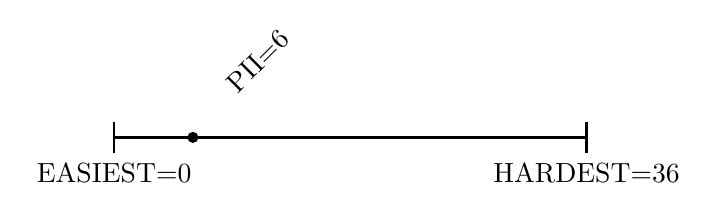
\begin{tikzpicture}[
        dot/.style = {circle, fill=black,inner sep=0pt, minimum size=4pt},
        every label/.append style = {inner sep=0pt, rotate around={45:(-0.5,1.5)}},
            thick      
    ]
        \draw (0,0.2) -- + (0,-0.4) node[below] {EASIEST=0};
        \draw (6,0.2) -- + (0,-0.4) node[below] {HARDEST=36};
        \draw[thick] (0,0) -- node[below=2mm] {} + (6,0);
        \node[dot,label={PII=6}] at (1,0) {};
    \end{tikzpicture}

    \caption{Portability Impediment Index \todo{fixme}}
    \label{fig:PII}
\end{figure}


\subsubsection{Human Factors Index}

Software programs are byproducts of human activities than incorporate our
problem-solving capabilities, cognitive aspects and social
interaction~\cite{b5}, therefore it is vital to understand what role did the
human factors play in our porting so that we can assess the quality of the
porting process. 

\todo{what do the numbers mean?}
In our case $\alpha_h = 2 + (-1) + 2 + 1 + 2 = 6$. As seen in
Figure~\ref{fig:HFI}, the HFI has a score very close to the lowest possible
score. Indeed, the human factor played a major role in our porting process, let
us analyze each factor and see what went wrong.

\begin{figure}
    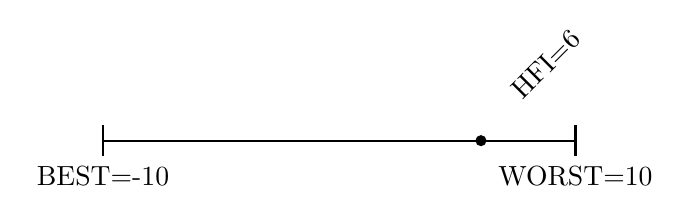
\begin{tikzpicture}[
        dot/.style = {circle, fill=black,inner sep=0pt, minimum size=4pt},
        every label/.append style = {inner sep=0pt, rotate around={45:(-0.5,1.5)}},
            thick      
    ]
        \draw (0,0.2) -- + (0,-0.4) node[below] {BEST=-10};
        \draw (6,0.2) -- + (0,-0.4) node[below] {WORST=10};
        \draw[thick] (0,0) -- node[below=2mm] {} + (6,0);
        \node[dot,label={HFI=6}] at (4.8,0) {};
    \end{tikzpicture}

    \caption{Human Factors Index \todo{fixme}}
    \label{fig:HFI}
\end{figure}

\textit{Knowledge about the program to be ported functions and structures (H1)} 
\todo{i don't like the "my" part}
As this was my first interaction with the program to be ported it was hard to
familiarize with its functions and structures, therefore I had no experience
whatsoever with the use cases of the program. This resulted in the inability to
easily solve the porting problems that appeared in our way.

\textit{Knowledge about the hardware and OS of the target system (H2)}
Hardware disparities were not a big concern in our porting as we used a portable
operating system and programming language that abstracted out hardware problems.
Therefore the focus was on the target operating system. Our porting moved the
program from an older version of Linux to a newer one. This helped us as we
did not have to learn the peculiarities of another operating system so that we
could finish our porting. However there were some problems that we faced
regarding the target operating system that we solved relatively straight
forward.

\textit{Knowledge and experience in the area of software porting (H3)}
As the experience of software porting was lacking there were many situations
and problems that could have been solved better, for example: doing better
tracking of the porting process, putting more effort in technical discussions
in order to better understand the problems, etc.

\textit{Knowledge of and experience with the language and program to be ported
in use(H4)}
The experience with the programming language (C++) helped us to grow the
productivity of the porting process as we did not have to care about low-level
impediments as endianness or data alignment. However we did have problems with
the language specification between different compilation toolchains that costed
us a whole week to solve. Finally, the experience with use cases of the program
to be ported was lacking. \todo{continue the ideas about the last phrase}

\textit{Knowledge about the functions and usage of tools used in the development
and testing environment (H5)}
While working in the development and testing environments we used a considerable
number of technologies, some of them being either new or not trivial to work
with. Here is a short list of these technologies: QEMU networking, SCons build
system, Perforce versioning system and internal tools as packaging system.
\todo{continue the ideas about the last phrase}

In retrospect, it seems that if the human factor index had a better score, maybe
the porting process would have lasted less and the problems we faced would not
even occur. \todo{fixme}

\subsubsection{Environmental Factors Index}

\todo{add intro}
In our porting we did not use any kind of unit testing so we will discard E2
from our discussion.

In the development environment we had no documentation describing the compiling
and linking procedures and no documentation regarding the environment dependent
components that we need to modify in order to move the code to a new
environment. We modified the code and the build system by trial and error. This
reduces the score for E1 as this strategy might not always work or it could take
an unsatisfactory amount of time for large and complicated systems. However
we managed to understand the peculiarities of the development environment and
get the first builds available for testing in two or three weeks, which is less
than 25\% of our porting time.

In the testing environment we had test programs and tools available such as
emulators and debuggers, furthermore the file transfer and conversion tools
were available from the start of the project. This facilitated the testing of
our program to be ported by allowing us to focus on the porting inconsistencies
rather than on testing infrastructure. Things were not perfect however, we did
have problems with the testing infrastructure that we solved in a short period
of time (\todo{add reference to porting difficulties} ).

That being said, the environmental factors index has the following value in our
case: \todo{what do these numbers mean?} $\alpha_e = 0 + NA + -1 = -1$. As seen in Figure~\ref{fig:EFI} we are in the
satisfactory half of the index, meaning that even if we had some difficulties
setting and understanding the development and testing environment, we managed
to work with them in order to achieve our goals.

\begin{figure}
    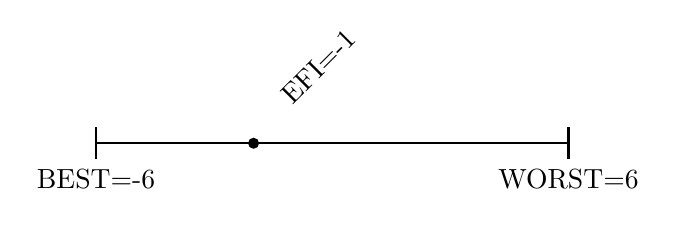
\begin{tikzpicture}[
        dot/.style = {circle, fill=black,inner sep=0pt, minimum size=4pt},
        every label/.append style = {inner sep=0pt, rotate around={45:(-0.5,1.5)}},
            thick      
    ]
        \draw (0,0.2) -- + (0,-0.4) node[below] {BEST=-6};
        \draw (6,0.2) -- + (0,-0.4) node[below] {WORST=6};
        \draw[thick] (0,0) -- node[below=2mm] {} + (6,0);
        \node[dot,label={EFI=-1}] at (2,0) {};
    \end{tikzpicture}

    \caption{Environmental Factors Index \todo{fixme}}
    \label{fig:EFI}
\end{figure}

\todo{ending thoughts}

\chapter{Discussions on Porting Costs} \label{sec:discussion}

% What I want to say in this section:
%   - I want to reflect on imporving the porting process we did. Tanaka proposes
%   the following seven ways of raising porting efficiency:
%     - porting guidlines
%     - porting compatibility checking tool
%     - portability evaluation tool
%     - tool for generating system calling routines
%     - program structure viewing tool
%     - os emulator
%     - test support tools
%   - I would like to see how relevant are they for our project. there is no way
%   at the moment to actually test the ways of improving porting efficiency so
%   I will keep the statements at the level of discussion, thinking about how
%   would have the process been different if we used one of the above ways (this
%   is chapter 3.2 from Tanaka)

% Subjects for discussion:
%  - the porting tasks affect each other in a non linear fashion
%  - we had errors in our extraction of costs from tracking
%  - it would be nice to have a dependency graph for the porting tasks. however
%  we could try to sketch some dependencies and see if an imporvement on one
%  side affects the other side
%  - what where the limitations in implementations and how do the improvements
%  from Tanaka apply to them
%  - compare our porting costs with the Table from Tanaka
%
%  - what does it mean to have an universal computer interface that would remove
%  any porting whatsoever (this discussion is in ../src -> background section if
%  i remember correctly)

\todo{split this text into subchapters}

In this section we present observations about the porting process and the
porting costs, focusing on the limitations of the porting model we used and on a
comparison between our results and the results of Tanaka et al.

Let us start by discussing the limitations of the porting model we proposed in
section~\ref{sec:background}. The model assumes that the tasks are executed in
sequential order, which is not true. The tasks are rather executed in a
non-linear fashion. For example while building for the target environment,
installing the binaries in this environment and testing the ported application,
we also had discussions about the difficulties and errors we encountered so that
we could later come back and solve the inconsistencies. However there was no
easy way to describe this dynamic so we chose to represent the task as they
would come one after another. The non-linearity of this porting model causes
problems while computing the porting costs. If one wants to compute the costs
with minimum error it means that more time must be allocated to the
\textit{Progress tracking} subtask. This strategy might not bring the best
results if the fixed total time of porting is computed in advance because
allocating more time for progress tracking means that other porting tasks must
have lesser time allocated. A good strategy here would compute first the
accepted error of man-hours present in the final porting costs so that an
acceptable ammount of time is allocated for tracking the progress of the
project. For our porting process it was not vital to have a small error in the
porting costs, we were interested to see an approximative distribution of time
per tasks so that we could answer questions as: where did we spend most time and
why? or what was the relation between development and testing? For this we
allocated an hour each week for tracking the status of the project, the planned
objectives for the future and the major difficulties we met in the respective
week. It is unclear, however, if more time spent on progress tracking would
improve the quality of other tasks. We can only guess, but more time spent on
tracking the working hours would mean that the developer has a better sense of
the time spent on each task, thus better managing multiple tasks at a time in
the future.

As discussed above, we had errors while extracting the porting costs for each
subtask in Table~\ref{tab:manHoursEvaluation}. There are two reasons for this
issue: the progress tracking format did not help us to extract the costs
correctly or the model we used for extracting the porting costs was not correct.
Firstly, the progress tracking format should have an intrinsic expresiveness that would
make it easy for the user to express the non-linearity of the porting tasks. To
create this kind of format we need to first find a way to describe the
non-linearity of the porting process, which is not a trivial task whatsoever.
Secondly, we expect a conversion error from the classical progress tracking
format (i.e., list of bullets for current status and planning) to the porting
model presented in section~\ref{sec:background}. This happens because there is
no straightforward way of converting a bullet as "IM is booting, having config
issues" (this example is taken from our progress tracking) into clear and
independent porting tasks. This is subject to interpretation one might say that
this bullet might be broken down into the following porting tasks:
\begin{itemize}
        \item Reviewing inconsistencies between source and remote environments
        \item Testing in target environment
        \item Discussions
        \item Surveying target OS
\end{itemize}
while another would break the bullet down into the following porting tasks:
\begin{itemize}
        \item Reviewing inconsistencies between source and remote environments
        \item Testing in target environment
\end{itemize}
It very much depends on the human factors and how the developers decide to work
with the provided tools and systems. Furthermore, to have a more accurate
conversion there must be time considerents: how much time did we spent on this
bullet? and how do we divide this time between porting tasks?

The next discussion point focuses on the porting tasks dependency graph. It
would be very difficult to sketch a complete graph between all tasks, instead we
can focus on specific areas of the graph that are somehow easier to understand
and sketch. The first area is the dependency between \textit{Testing} and all
subtasks in \textit{Building for target environment}. There is a continous
feedback between the testing phase and the development phase. While porting we
built binaries, installed them on target environment, tested them and expected
to see errors of linking, problems with the installation or actual
inconsistencies and problems with dependencies that would be solved in a future
iteration of this process. This iterative process with continous feedback
between testing and development is a building block of the Agile methodology, if
we used other software methodology as Waterfall maybe the dependency would be
completely different. The second area we focus on is the dependency between
\textit{General duties} and all other subtasks. Documentation is linked to all
subtasks because we need to include all relevant information in the documents we
produce, progress tracking must reflect work executed in each subtask and
discussions are by design focused on trying to understand each part of the
porting process. That being said, it is hard to imagine how \textit{General
duties} would not be a substantial port of the porting process. It would be
interesting too see if a modification in the allocated time for a subtask such
as \textit{Discussions} would reduce or increase the needed time for other
subtasks, otherwise if other tasks are not affected by this modification, there
should be no interest in allocating more time for discussing.

At this moment we discussed the limitations and open problems that appear in the
model of porting we used. Next, we make a comparison between our results for
porting costs and the results that appeared in the first paper that presented a
basis for our porting model~\cite{b1}. The results can be found in Table 6 of
the paper we referenced. We will compare the subtotals per tasks and discuss the
reasons of the differences between the two . In terms of \textit{Advance
preparations} we spend a total of 14.35\% of our total time while Tanaka et al.
spend 33.4\%. There are two major reasons for reduced time in our case. First,
we were interested in delivering builds for the target environment as fast as
possible, sacrificing the time spent on understanding each part of the system we
were trying to port. We found no easy way to understand the components of the
system by surveying the documentation and the program for porting so we decided
to offload this work on the build system (i.e., when the compiler threw errors
for a component, we went to that component, understood it and solved the
problems). Second, we worked with the Agile methodology in mind, combining
subtasks from different tasks in the same iteration. For this reason we
losed the focus on the \textit{Advance preparations} because we were also
interested in subtasks from \textit{Building for target environment}, for
example. Tanaka et al. seem to work with a Waterfall methodology. This might
explain the increased time in this initial stage.

Next we compare the \textit{Building for target environment} in our model with
\textit{Target testing} from Tanaka et al. There are significant differences in
the subtasks from the two models but we are interested in a comparison of
development time (i.e., actual work focused on solving errors and
inconsistencies, building binaries, etc.). It seems that Tanaka et al. put the
time spent on solving errors and the time spent on testing in the same category.
This makes the comparison difficult as we do not know how to divide this time.
However our time spent in this stage is 32.71\% while Tanaka et al. spend
27.8\%. The most time consuming task for us was to work with the build system,
which is not the case for them. This shows the major difference between our
project and theirs. While our porting was focused on extracting components from
a larger ecosystem into a target environment, their project was focused on
porting a whole application from one environment to another.

For \textit{Testing} we assume that they spent $\textit{Linked test on target} /
2 + \textit{Workstation testing} = 10.5 + 11.4 = 21.9\%$. We dived the linked
test on target because we assumed that half of this time was allocated to
development and half of it was allocated to testing. Their time for
\textit{General duties} is of 27.4\%. These two times are very similar with our
project (i.e, 24.53\% and 28.26\%). This might mean that testing and general
duties represent a major part in each software porting project, thus when
evaluating the costs in advance, special attention must be payed to these tasks.

\todo{add some final words for this chapter}

\section{Conclusions and Further Work}

\subsection{Conclusions}
We succeeded in porting the IxOS infrastructure on ARM boards. We separated the
relevant components for our porting (i.e., InterfaceManager and IxStack) from
IxOS so that they run on every ARM-based Linux distribution. At the moment of
writing the project is in the proof-of-concept stage. If there is interest for
continuing the project or integrating it in other projects inside the company,
we provided the necessary environment for deploying it.

We have extracted the porting costs for porting IxOS infrastructure on ARM
boards. Thus we understood what the weaknesses and the strengths of our project
were. The lack of understanding of the project structure and project use cases
proved itself to be an important factor during the process of porting. Because
of this reason we had to spend additional time on testing the system and
understanding its components. This time might have been better allocated on
solving problems and inconsistencies. A strength of our project was the fact
that the program for porting had a high degree of portability. This helped us to
shrink the volume of inconsistencies between the source environment and the
target environment.

We succeeded in creating a better model for software porting starting from the
model presented in~\cite{b1,b2} and from our project specific needs. We
contributed to this model by making it more generic and allowing other software
porting projects to easily map their needs on this model.

Finally, we have provided a discussion on the limitations of the model we
created and provided a comparison between our porting results and the results
presented in the first work~\cite{b1} that came up with the model we used as a
basis for our generic porting model.

\subsection{Further Work}

We plan to test the performance of the system so that we can achieve the other
goal we proposed in the beginning of this work (i.e., explore Ixia testing
infrastructure on other architectures so that we can achieve a better
performance of the system). To achieve this goal we will compare our solution in
the target environment with the same solution in the source environment. We
expect to see better results in the new environment for some network testing
suites than in the old environment. Furthermore, we plan to compare our solution
with other open-source network testing tools.

To complete the analysis of the factors that affected the porting costs we plan
to analyze the characteristics of the program to be ported. We want to analyze
the program size and contents and the content of the changes needed for porting.
By doing this we hope to find a direct correspondence between the program to be
ported and specific porting subtasks (e.g., \textit{Solving inconsistencies
between source and target environment}).

Finally, we want to analyze the porting improvements guidelines presented
in~\cite{b1} and map them on our porting process. However, we do not plan to
restart the porting process while mapping these guidelines, instead we want to
have a discussion and draw conclusions based on them.


\begin{thebibliography}{00}
\bibitem{b1} Tanaka, T.; Hakuta, M.; Iwata, N.; Ohminami, M. (1995). [IEEE Comput. Soc. Press 12th TRON Project International Symposium - Tokyo, Japan (28 Nov.-2 Dec. 1995)] Proceedings of the 12th TRON Project International Symposium - Approaches to making software porting more productive. , (), 73–85.
\bibitem{b2} Mitsuari Hakuta; Masato Ohminami (1997). A study of software portability evaluation. , 38(2), 145–154.
\bibitem{b3} L. Fernando Capretz, "Bringing the Human Factor to Software Engineering" in IEEE Software, vol. 31, no. 02, pp. 104-104, 2014.
\bibitem{b4} A. Kanai, T. Furuyama and M. Takahashi, "A cost model for software conversion based on program characteristics and a converter effect," [1992] Proceedings. The Sixteenth Annual International Computer Software and Applications Conference, 1992, pp. 63-68
\bibitem{b5} Mooney, J.D., 2004. Developing portable software. In Information Technology (pp. 55-84). Springer, Boston, MA.
\bibitem{b6} Ejiogu, L.O., 1985. A simple measure of software complexity. ACM SIGPLAN Notices, 20(3), pp.16-31.
\end{thebibliography}

\end{document}
